% ============================================================================
% REQUIRED PACKAGES & CONFIGURATIONS FOR COMPILING THIS EXPERIMENT:
% ----------------------------------------------------------------------------
% \usepackage{circuitikz}      % For drawing IC 555 timer schematics
% \usepackage{pgfplots}        % For plotting charging/discharging & output waveforms
% \pgfplotsset{compat=1.18}    % Ensures modern rendering engine defaults
% \usepackage{booktabs}        % For publication-grade tables
% \usepackage{amsmath}         % For mathematical expressions
% \usepackage{siunitx}         % For standard units (\SI, \kilo\ohm, \micro\farad)
% \usepackage{subcaption}      % For multi-panel figures
% ============================================================================

\chapter{Astable Multivibrator Using IC 555}

\section{Aim}
To design, construct, and evaluate an Astable Multivibrator (Free-Running Oscillator) circuit using the IC 555 timer for the given frequency and duty ratio specifications. %The specific objectives are:
\begin{enumerate}
	\item To observe and record the output square wave and timing capacitor exponential charge/discharge voltage waveforms on a Digital Storage Oscilloscope (DSO).
	\item To measure the high time ($t_1$), low time ($t_2$), overall time period ($T$), output frequency ($f_0$), and duty cycle ($D$).
	\item To verify upper ($V_{TH}$) and lower ($V_{TL}$) trigger thresholds relative to the supply voltage $V_{CC}$.
	\item To compare experimentally measured timing parameters with theoretical values derived from component values.
\end{enumerate}

\section{Pre-Lab Assignment}
Before conducting the laboratory session, complete the following analytical problems:
\begin{enumerate}
	\item Sketch the internal block diagram of IC 555 showing the voltage divider network, two comparators, RS flip-flop, discharge transistor, and output driver stage.
\item Derive the expressions for the capacitor charging time ($t_1$), discharging time ($t_2$), total time period ($T$), frequency ($f_0$), and duty cycle ($D$) for an astable multivibrator.
\item Calculate $R_A$, $R_B$, and $C$ required to generate a square wave of $f_0 = 1\text{ kHz}$ with a duty cycle $D = 66.7\%$ using a supply voltage of $V_{CC} = +5\text{ V}$.
\item Explain why a standard 555 astable multivibrator circuit cannot achieve a duty cycle of $50\%$ or less, and describe how a steering diode can be added to achieve a $50\%$ duty cycle.
\end{enumerate}

\section{Components and Equipment Required}
The required components and test instruments are listed in Table \ref{tab:components_astable555}.

\begin{table}[h!]
\centering
\caption{Components and Equipment Specifications}
\label{tab:components_astable555}
\begin{tabular}{llll}
	\toprule
	\textbf{S. No.} & \textbf{Item Name} & \textbf{Specification / Range} & \textbf{Quantity} \\
	\midrule
	1 & Timer IC & IC 555 (8-pin DIP) & 1 No. \\
	2 & Resistors & \SI{4.7}{\kilo\ohm} (1\% Tolerance) & 2 Nos. \\
	3 & Timing Capacitor & \SI{0.1}{\micro\farad} (Ceramic/Film) & 1 No. \\
	4 & Bypass Capacitor & \SI{0.01}{\micro\farad} (Ceramic) & 1 No. \\
	5 & Regulated DC Power Supply & $+5\text{ V}$ or $+12\text{ V}$ DC & 1 No. \\
	6 & Digital Storage Oscilloscope & Dual Channel, \SI{20}{\mega\hertz} or higher & 1 No. \\
	7 & Digital Multimeter & $4\frac{1}{2}$ digit display & 1 No. \\
	8 & Breadboard \& Wires & Standard setup & As required \\
	\bottomrule
\end{tabular}
\end{table}

\section{Theory}
An astable multivibrator is a regenerative circuit with two quasi-stable states. It oscillates continuously between these states without requiring external triggering. When constructed using the IC 555 timer, timing is controlled by an external RC network ($R_A$, $R_B$, and $C$).

\subsection{Principle of Operation}
The internal voltage divider of the 555 IC sets reference thresholds of $V_{TH} = \frac{2}{3} V_{CC}$ for Comparator 1 (Threshold) and $V_{TL} = \frac{1}{3} V_{CC}$ for Comparator 2 (Trigger).

\begin{itemize}
\item \textbf{Charging Phase (High Output State):} Initially, capacitor $C$ is uncharged ($V_C < \frac{1}{3} V_{CC}$). Comparator 2 sets the internal RS flip-flop, forcing Output (Pin 3) HIGH ($V_{OH} \approx V_{CC}$) and turning the internal discharge transistor (Pin 7) OFF. Capacitor $C$ charges exponentially towards $V_{CC}$ through resistors $R_A$ and $R_B$. The charging time $t_1$ required for $V_C$ to rise from $\frac{1}{3} V_{CC}$ to $\frac{2}{3} V_{CC}$ is:
\begin{equation}
	t_{ON} = \ln(2) \cdot (R_A + R_B) C \approx 0.693 (R_A + R_B) C
\end{equation}

\item \textbf{Discharging Phase (Low Output State):} When $V_C$ reaches $\frac{2}{3} V_{CC}$, Comparator 1 resets the flip-flop, driving Output (Pin 3) LOW ($V_{OL} \approx 0\text{ V}$) and turning the discharge transistor (Pin 7) ON (connecting it to GND). Capacitor $C$ discharges exponentially towards $0\text{ V}$ through $R_B$ into Pin 7. The discharge time $t_2$ required for $V_C$ to fall from $\frac{2}{3} V_{CC}$ to $\frac{1}{3} V_{CC}$ is:
\begin{equation}
	t_{OFF} = \ln(2) \cdot R_B C \approx 0.693 R_B C
\end{equation}
\end{itemize}

\subsection{Frequency and Duty Cycle Derivations}
The total period of oscillation $T$ is the sum of charging and discharging durations:
\begin{equation}
T = t_{ON} + t_{OFF} = 0.693 (R_A + 2 R_B) C
\end{equation}
The overall frequency of oscillation $f$ is given by:
\begin{equation}
f = \frac{1}{T} = \frac{1.44}{(R_A + 2 R_B) C}
\end{equation}
The duty cycle $D$, defined as the ratio of HIGH output duration to total period, is:
\begin{equation}
D = \frac{t_1}{T} \times 100\% = \frac{R_A + R_B}{R_A + 2 R_B} \times 100\%
\end{equation}
Since $R_A > 0$, $D$ is always strictly greater than $50\%$\footnote{There are ways in which duty ratio $D\le 50\%$ can be achieved.}.

\section{Circuit Diagram}
The schematic for the 555 Astable Multivibrator circuit is presented in Figure \ref{fig:555_astable_schematic}.

\begin{figure}[h!]
\centering
\begin{circuitikz}[scale=0.9, transform shape]
	% Draw IC 555 Main Block
	\draw (0,0) rectangle (4.5,5);
	\node at (2.25,2.5) {\Large \textbf{IC 555}};
	
	% Pin Labels inside box
	\node[right, font=\footnotesize] at (0,4.2) {4: RESET};
	\node[right, font=\footnotesize] at (0,3.2) {7: DISCH};
	\node[right, font=\footnotesize] at (0,2.0) {6: THRES};
	\node[right, font=\footnotesize] at (0,0.8) {2: TRIG};
	\node[left, font=\footnotesize]  at (4.5,4.2) {8: $V_{CC}$};
	\node[left, font=\footnotesize]  at (4.5,2.5) {3: OUT};
	\node[left, font=\footnotesize]  at (4.5,0.8) {5: CTRL};
	\node[above, font=\footnotesize] at (2.25,0) {1: GND};
	
	% Power Supply Rail (+5V)
	\draw (-3,5.5) node[above] {$+V_{CC}\ (+5\text{V})$} -- (6,5.5);
	\draw (-3,5.5) node[circle, fill, inner sep=1.5pt] {} to[short] (-3,5.5);
	
	% Connect Pin 8 (VCC) and Pin 4 (RESET) to Power Rail
	\draw (4.5,4.2) -- (5.2,4.2) -- (5.2,5.5) node[circ] {};
	\draw (0,4.2) -- (-2.0,4.2) -- (-2.0,5.5) node[circ] {};
	
	% Connect Pin 1 (GND) to Ground Rail
	\draw (2.25,0) -- (2.25,-1.2) node[ground] {};
	
	% Bypass Capacitor at Pin 5 (Control Voltage)
	\draw (4.5,0.8) -- (5.5,0.8) to[C, l=$C_2\ (\SI{0.01}{\micro\farad})$] (5.5,-1.2) node[ground] {};
	
	% Resistors RA and RB along timing network
	\draw (-3,5.5) to[R, l_=$R_A\ (\SI{2.7}{\kilo\ohm})$] (-3,3.2) node[circ] (node7) {};
	\draw (node7) -- (0,3.2);
	
	\draw (node7) to[R, l_=$R_B\ (\SI{5.6}{\kilo\ohm})$] (-3,1.4) node[circ] (node62) {};
	
	% Tie Pin 6 and Pin 2 together
	\draw (node62) -- (-1.2,1.4) -- (-1.2,2.0) -- (0,2.0);
	\draw (-1.2,1.4) -- (-1.2,0.8) -- (0,0.8);
	
	% Timing Capacitor C
	\draw (node62) to[C, l_=$C\ (\SI{0.1}{\micro\farad})$] (-3,-1.2) node[ground] {};
	
	% Output Connection (Pin 3)
	\draw (4.5,2.5) -- (6.0,2.5) node[circ] {} node[right] {$V_{out}$};
	
	% Node labels for oscilloscope measurement
	\node[left] at (-3,1.4) {$V_C$};
\end{circuitikz}
\caption{IC 555 Astable Multivibrator Schematic}
\label{fig:555_astable_schematic}
\end{figure}

\section{Design}
\subsection{Design Specifications}
\begin{itemize}
	\item Target Output Frequency: $f_0 = 1\text{ kHz} \implies T = 1.0\text{ ms}$
	\item Target Duty Cycle: $D = 60\% = 0.60$
	\item Power Supply Voltage: $V_{CC} = +5\text{ V DC}$
	\item Chosen Timing Capacitor: $C = \SI{0.1}{\micro\farad}$
\end{itemize}

\subsection{Calculations}
\subsubsection{Timing Equations}
\begin{itemize}
	\item \textbf{High Output Duration ($t_{ON}$):} Capacitor charges from $\frac{1}{3} V_{CC}$ to $\frac{2}{3} V_{CC}$:
	\begin{equation}
		t_{ON} = \ln(2) \cdot (R_A + R_B) C \approx 0.693 (R_A + R_B) C
	\end{equation}
	
	\item \textbf{Low Output Duration ($t_2$):} Capacitor discharges from $\frac{2}{3} V_{CC}$ to $\frac{1}{3} V_{CC}$:
	\begin{equation}
		t_{OFF} = \ln(2) \cdot R_B C \approx 0.693 R_B C
	\end{equation}
	
	\item \textbf{Total Time Period ($T$) and Frequency ($f_0$):}
	\begin{equation}
		T = t_{ON} + t_{OFF} = 0.693 (R_A + 2 R_B) C
	\end{equation}
	\begin{equation}
		f_0 = \frac{1}{T} = \frac{1.44}{(R_A + 2 R_B) C}
	\end{equation}
\end{itemize}
\begin{enumerate}
	\item Determine resistor ratio for $D = 0.60$:
	\begin{equation}
		R_A = \left( \frac{2(0.60) - 1}{1 - 0.60} \right) R_B = \left( \frac{0.20}{0.40} \right) R_B = 0.5 R_B \implies R_B = 2 R_A
	\end{equation}
	
	\item Express total period $T$ in terms of $R_B$:
	\begin{equation}
		T = 0.693 (0.5 R_B + 2 R_B) C = 0.693 (2.5 R_B) C = 1.7325 \cdot R_B C
	\end{equation}
	
	\item Calculate target $R_B$ and $R_A$:
	\begin{equation}
		R_B = \frac{T}{1.7325 \cdot C} = \frac{1.0 \times 10^{-3}\text{ s}}{1.7325 \times (0.1 \times 10^{-6}\text{ F})} \approx 5772\ \Omega = \SI{5.77}{\kilo\ohm}
	\end{equation}
	\begin{equation}
		R_A = 0.5 \cdot R_B = \SI{2.89}{\kilo\ohm}
	\end{equation}
	
	\item Select nearest standard E12 resistor values:
	\begin{equation}
		R_A = \SI{2.7}{\kilo\ohm}, \quad R_B = \SI{5.6}{\kilo\ohm}
	\end{equation}
	
	\item Recalculate the expected parameters with the selected standard components:
	\begin{equation}
		t_1 = 0.693 \times (2.7\text{ k}\Omega + 5.6\text{ k}\Omega) \times 0.1\ \mu\text{F} = 0.575\text{ ms}
	\end{equation}
	\begin{equation}
		t_2 = 0.693 \times (5.6\text{ k}\Omega) \times 0.1\ \mu\text{F} = 0.388\text{ ms}
	\end{equation}
	\begin{equation}
		T_{\text{design}} = 0.575\text{ ms} + 0.388\text{ ms} = 0.963\text{ ms}
	\end{equation}
	\begin{equation}
		f_{0,\text{design}} = \frac{1}{0.963 \times 10^{-3}\text{ s}} \approx 1038.4\text{ Hz} \quad (1.04\text{ kHz})
	\end{equation}
	\begin{equation}
		D_{\text{design}} = \frac{2.7 + 5.6}{2.7 + 2(5.6)} \times 100\% = \frac{8.3}{13.9} \times 100\% = 59.71\% \approx 60\%
	\end{equation}
\end{enumerate}

\section{Procedure}
\begin{enumerate}
	\item Assemble the circuit on a breadboard using $R_A = \SI{2.7}{\kilo\ohm}$, $R_B = \SI{5.6}{\kilo\ohm}$, and $C = \SI{0.1}{\micro\farad}$ according to Figure \ref{fig:555_astable_schematic}.
	\item Connect a bypass capacitor $C_2 = \SI{0.01}{\micro\farad}$ between Pin 5 and GND to suppress noise pickup.
	\item Apply $+5\text{ V}$ DC power to Pin 8 and Pin 4, and ground Pin 1.
	\item Connect Channel 1 of the DSO to $V_C$ (Pins 2/6) and Channel 2 to $V_{out}$ (Pin 3).
	\item Set DSO channels to DC coupling and adjust timebase to display 2 to 3 full cycles.
	\item Measure high time $t_1$, low time $t_2$, upper threshold $V_{TH}$, and lower threshold $V_{TL}$.
	\item Calculate practical period $T = t_1 + t_2$, frequency $f_0 = 1/T$, and duty cycle $D = (t_1/T) \times 100\%$.
\end{enumerate}

\section{Precautions}
\begin{enumerate}
	\item Ensure Pin 4 (RESET) is connected directly to $+V_{CC}$ to avoid spontaneous resetting.
	\item Use non-polarized ceramic or film capacitors for timing capacitor $C$.
	\item Ensure all ground leads from power supply and DSO probes share a single common ground node.
\end{enumerate}

\section{Model Graph / Expected Waveforms}
Figure \ref{fig:555_expected_waveforms} illustrates the expected time-aligned output square wave ($V_{out}$) and capacitor exponential charge/discharge waveform ($V_C$) for a $60\%$ duty cycle design.

\begin{figure}[h!]
	\centering
	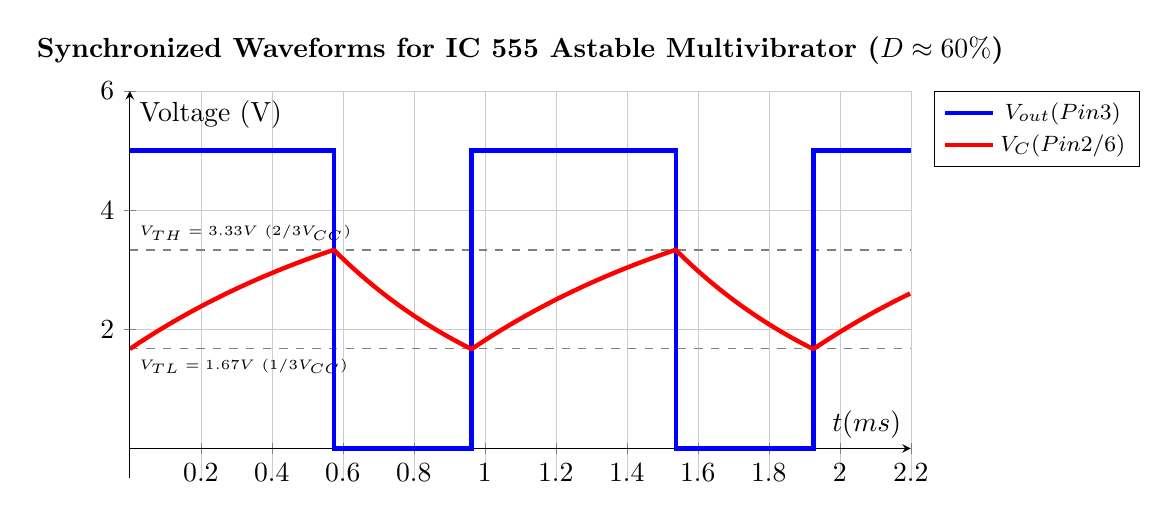
\begin{tikzpicture}
		\begin{axis}[
			use fpu=false,
			axis lines=middle,
			xlabel={$t\text{ (ms)}$},
			ylabel={Voltage (V)},
			xmin=0, xmax=2.2,
			ymin=-0.5, ymax=6.0,
			grid=both,
			grid style={line width=.1pt, draw=gray!20},
			major grid style={line width=.2pt, draw=gray!40},
			width=11.5cm, height=6.5cm,
			title={\textbf{Synchronized Waveforms for IC 555 Astable Multivibrator ($D \approx 60\%$)}},
			legend pos=outer north east,
			legend style={font=\footnotesize},
			% Define the piecewise logic using declare function
			declare function={
				T = 0.963;          % Total period
				t1 = 0.575;         % High time (charging phase)
				t_rel(\t) = mod(\t, T); % Time relative to the current period start
				% Piecewise capacitor formula:
				Vc(\t) = (t_rel(\t) < t1) ? 
				(5 - (5 - 1.67)*exp(-1.205*t_rel(\t))) : 
				(3.33*exp(-1.786*(t_rel(\t) - t1)));
			}
			]
			% Threshold Lines
			% 1. Threshold Line 1 (Excluded from legend using "forget plot")
			\addplot[gray, dashed, domain=0:2.2, forget plot] {3.33};
			\node[font=\tiny, above right] at (axis cs: 0, 3.33) {$V_{TH} = 3.33\text{V}\ (2/3 V_{CC})$};
			% 2. Threshold Line 2 (Excluded from legend using "forget plot")
			\addplot[gray, dashed, domain=0:2.2, forget plot] {1.67};
			\node[font=\tiny, below right] at (axis cs: 0, 1.67) {$V_{TL} = 1.67\text{V}\ (1/3 V_{CC})$};
			
			% Output Waveform Vout (High: 5V, Low: 0V, t1=0.575ms, t2=0.388ms, T=0.963ms)
			\addplot[ultra thick, blue] coordinates {
				(0, 5) (0.575, 5) (0.575, 0) (0.963, 0)
				(0.963, 5) (1.538, 5) (1.538, 0) (1.926, 0) (1.926, 5) (2.2, 5)
			};
			\addlegendentry{$V_{out}\text{ (Pin 3)}$}
			
			% Capacitor Voltage VC Exponential Charging & Discharging
			% Single \addplot command for the entire waveform
			\addplot[ultra thick, red, domain=0:2.2, samples=400] {Vc(x)};
			\addlegendentry{$V_C\text{ (Pin 2/6)}$}
			%	\addplot[ultra thick, red, domain=0:{0.575}, samples=50] {5 - (5 - 1.67)*exp(-1.205*x)};
			%	\addplot[ultra thick, red, domain={0.575}:{0.963}, samples=50] {3.33*exp(-1.786*(x-0.575))};
			%	\addplot[ultra thick, red, domain={0.963}:{1.538}, samples=50] {5 - (5 - 1.67)*exp(-1.205*(x-0.963))};
			%	\addplot[ultra thick, red, domain={1.538}:{1.926}, samples=50] {3.33*exp(-1.786*(x-1.538))};
			%	\addplot[ultra thick, red, domain={1.926}:{2.2}, samples=50] {5 - (5 - 1.67)*exp(-1.205*(x-1.926))};
			%	\addlegendentry{$V_C\text{ (Pin 2/6)}$}
		\end{axis}
	\end{tikzpicture}
	\caption{Model Output and Capacitor Voltage Waveforms for 60\% Duty Ratio Design}
	\label{fig:555_expected_waveforms}
\end{figure}

\section{Observation Tables}

\subsection{Waveform Parameters}
Record timing and frequency parameters in Table \ref{tab:obs_astable_timing}.

\begin{table}[h!]
	\centering
	\caption{Theoretical vs Practical Waveform Measurements}
	\label{tab:obs_astable_timing}
	\begin{tabular}{lcccc}
		\toprule
		\textbf{Parameter} & \textbf{Theoretical Value} & \textbf{Measured Value} & \textbf{\% Error} \\
		\midrule
		High Time ($t_1$) & $0.575\text{ ms}$ & & \\
		Low Time ($t_2$) & $0.388\text{ ms}$ & & \\
		Time Period ($T$) & $0.963\text{ ms}$ & & \\
		Frequency ($f_0$) & $1038.4\text{ Hz}$ & & \\
		Duty Cycle ($D$) & $59.71\%$ & & \\
		\bottomrule
	\end{tabular}
\end{table}

\section{Result}
The IC 555 astable multivibrator was designed and tested for a target $60\%$ duty ratio:
\begin{itemize}
	\item Measured high time $t_1 = \rule{1.8cm}{0.15mm}\text{ ms}$ and low time $t_2 = \rule{1.8cm}{0.15mm}\text{ ms}$, giving a practical time period $T = \rule{1.8cm}{0.15mm}\text{ ms}$.
	\item The experimental duty cycle was calculated as $D_{\text{practical}} = \rule{1.8cm}{0.15mm}\%$ (Theoretical: $59.71\%$, target: $60\%$).
	\item Output oscillation frequency was measured as $f_{0,\text{practical}} = \rule{1.8cm}{0.15mm}\text{ Hz}$ compared to the theoretical value of $1038.4\text{ Hz}$.
\end{itemize}

\section{Questions}
\begin{enumerate}
	\item How can a steering diode connected across $R_B$ enable independent adjustment of duty cycles below $50\%$?
	\item What are the upper and lower limits on duty cycle $D$ achievable with the standard 555 astable topology without steering diodes?
	\item How can an astable 555 multivibrator circuit be modified to get a $50\%$ duty cycle square wave?
	\item How does replacing $R_A$ and $R_B$ with a potentiometer affect the frequency and duty cycle?
	\item What is the effect on output duty cycle if supply voltage $V_{CC}$ fluctuates between $+5\text{ V}$ and $+12\text{ V}$?
	%\item Compare the performance of the bipolar IC 555 with the CMOS equivalent (e.g., LMC555) in terms of minimum operating voltage and maximum timing resistor limits.

	\item What happens to the oscillation frequency and output amplitude if the supply voltage $V_{CC}$ is increased from $+5\text{ V}$ to $+12\text{ V}$? Explain why.
	\item What is the functional role of Pin 5 (Control Voltage), and how can it be used to achieve frequency modulation (FM)?
\item Why does the timing capacitor $C$ charge through $(R_A + R_B)$ but discharge only through $R_B$?
\item Compare the IC 555 astable multivibrator with an op-amp relaxation oscillator in terms of frequency stability and output driving capability.
\end{enumerate}